\documentclass[11pt]{article}

%% MinionPro fonts 
%\usepackage[lf]{MinionPro}
%\usepackage{MnSymbol}
\usepackage{microtype}

%% Margins
\usepackage{geometry}
\geometry{verbose,letterpaper,tmargin=1in,bmargin=1in,lmargin=1in,rmargin=1in}

%% Other packages
\usepackage{amsmath}
\usepackage{amsthm}
\usepackage[shortlabels]{enumitem}
\usepackage{titlesec}
\usepackage{soul}
\usepackage{tikz}
\usepackage{mathtools}
\usepackage{pgfplots}
\usepackage{tikz-3dplot}
\usepackage{algorithmic}
\usepackage[export]{adjustbox}
\usepackage{tcolorbox}
\usepackage{optprog}
\usepackage{amsfonts}
\usepackage{pdfpages}

%% Paragraph style settings
\setlength{\parskip}{\medskipamount}
\setlength{\parindent}{0pt}

%% Change itemize bullets
\renewcommand{\labelitemi}{$\bullet$}
\renewcommand{\labelitemii}{$\circ$}
\renewcommand{\labelitemiii}{$\diamond$}
\renewcommand{\labelitemiv}{$\cdot$}

%% Colors
\definecolor{rred}{RGB}{204,0,0}
\definecolor{ggreen}{RGB}{0,145,0}
\definecolor{yyellow}{RGB}{255,185,0}
\definecolor{bblue}{rgb}{0.2,0.2,0.7}
\definecolor{ggray}{RGB}{190,190,190}
\definecolor{ppurple}{RGB}{160,32,240}
\definecolor{oorange}{RGB}{255,165,0}

%% Shrink section fonts
\titleformat*{\section}{\normalsize\bf}
\titleformat*{\subsection}{\normalsize\bf}
\titleformat*{\subsubsection}{\normalsize\it}

% %% Compress the spacing around section titles
\titlespacing*{\section}{0pt}{1.5ex}{0.75ex}
\titlespacing*{\subsection}{0pt}{1ex}{0.5ex}
\titlespacing*{\subsubsection}{0pt}{1ex}{0.5ex}

%% amsthm settings
\theoremstyle{definition}
\newtheorem{problem}{Problem}
\newtheorem{example}{Example}
\newtheorem*{theorem}{Theorem}
\newtheorem*{bigthm}{Big Theorem}
\newtheorem*{biggerthm}{Bigger Theorem}
\newtheorem*{bigcor1}{Big Corollary 1}
\newtheorem*{bigcor2}{Big Corollary 2}

%% tikz settings
\usetikzlibrary{calc}
\usetikzlibrary{patterns}
\usetikzlibrary{decorations}
\usepgfplotslibrary{polar}


%% algorithmic setup
\algsetup{linenodelimiter=}
\renewcommand{\algorithmiccomment}[1]{\quad// #1}
\renewcommand{\algorithmicrequire}{\emph{Input:}}
\renewcommand{\algorithmicensure}{\emph{Output:}}

%% Answer box macros
%% \answerbox{alignment}{width}{height}
\newcommand{\answerbox}[3]{%
  \fbox{%
    \begin{minipage}[#1]{#2}
      \hfill\vspace{#3}
    \end{minipage}
  }
}

%% \answerboxfull{alignment}{height}
\newcommand{\answerboxfull}[2]{%
  \answerbox{#1}{6.38in}{#2} 
}

%% \answerboxone{alignment}{height} -- for first-level bullet
\newcommand{\answerboxone}[2]{%
  \answerbox{#1}{6.0in}{#2} 
}

%% \answerboxtwo{alignment}{height} -- for second-level bullet
\newcommand{\answerboxtwo}[2]{%
  \answerbox{#1}{5.8in}{#2}
}

%% special boxes
\newcommand{\wordbox}{\answerbox{c}{1.2in}{.7cm}}
\newcommand{\catbox}{\answerbox{c}{.5in}{.7cm}}
\newcommand{\letterbox}{\answerbox{c}{.7cm}{.7cm}}

%% Miscellaneous macros
\newcommand{\tstack}[1]{\begin{multlined}[t] #1 \end{multlined}}
\newcommand{\cstack}[1]{\begin{multlined}[c] #1 \end{multlined}}
\newcommand{\ccite}[1]{\only<presentation>{{\scriptsize\color{gray} #1}}\only<article>{{\small [#1]}}}
\newcommand{\grad}{\nabla}
\newcommand{\ra}{\ensuremath{\rightarrow}~}
\newcommand{\maximize}{\text{maximize}}
\newcommand{\minimize}{\text{minimize}}
\newcommand{\subjectto}{\text{subject to}}
\newcommand{\trans}{\mathsf{T}}
\newcommand{\bb}{\mathbf{b}}
\newcommand{\bx}{\mathbf{x}}
\newcommand{\bc}{\mathbf{c}}
\newcommand{\bd}{\mathbf{d}}
\newcommand{\blu}{\color{blue}}
%% LP format
%    \begin{align*}
%      \maximize \quad & \mathbf{c}^{\trans} \mathbf{x}\\
%      \subjectto \quad & A \mathbf{x} = \mathbf{b}\\
%                       & \mathbf{x} \ge \mathbf{0}
%    \end{align*}


%% Redefine maketitle
\makeatletter
\renewcommand{\maketitle}{
  \noindent SA405 -- AMP 

  \begin{center}\Large{\textbf{\@title}}\end{center}
}
\makeatother

\begin{document}

\title{HW6: Branch and Bound}

\maketitle

\begin{enumerate}

\item Solve the following problem using Branch and Bound

\begin{optprog*}
max & \objective{5 x_1 + 4x_2} \\
st & 6x_1 + 13 x_2 & \leq & 67 \\
   & 8 x_1 + 5x_2 & \leq & 55 \\
   & x_1, x_2 & \in & \mathbb{Z}^+
\end{optprog*}

Solve each subproblem graphically or with python.

{\blu
I solved each subproblem in Python. The branch and bound tree is on the next page. The logic is as follows.

\begin{itemize}
\item Step 1, solve P1. Initial solution $z = 36.8$, $x = (5.1,2.8)$. At this point, I know $z_{IP} \leq 36$. I can branch on either $x_1$ or $x_2$, I choose $x_1$
\item Step 2, solve P2 and P3. For P2, $z = 36.3$ and $x_2$ is fractional. For P3, $z = 35.6$, $x_2$ is fractional. I can branch on either P2 or P3. I choose P2 because $36.3 > 35.6$.
\item Step 3: Solve P4 and P5. For P4, $z = 33$ and solution is integer. For P5, $ z = 35.3$ and $x_1$ is fractional. So at this point, I know $33 \leq z_{IP} \leq 36$. I can choose to branch on either P3 or P5. I choose P3
\item Step 4: Solve P6 and P7. For P6, $z = 35.25$ and $x_1$ is fractional. P7 is infeasible. At this point, my active nodes are P5 and P6. Note that both have $z$ values between 35 and 36. So I can update my bounds to be $33 \leq z_{IP} \leq 35$. I choose to branch on P5.
\item Step 5: Solve P8 and P9. For P8, $z = 33.2$ and $x_2$ is fractional. P9 is infeasible. I eliminate node P8 because $33.2$ is equal to my current lower bound. All that's left is to branch on P6.
\item Step 6: Solve P10 and P11. For P10, $z = 34$ and is integral. P11 is infeasible. No active nodes are left. P10 becomes my current solution because $34 > 33$. I stop, P10 is optimal.
\end{itemize}

The optimal solution is $x^* = (6,1)$ with objective value $z^* = 34$.


\newpage
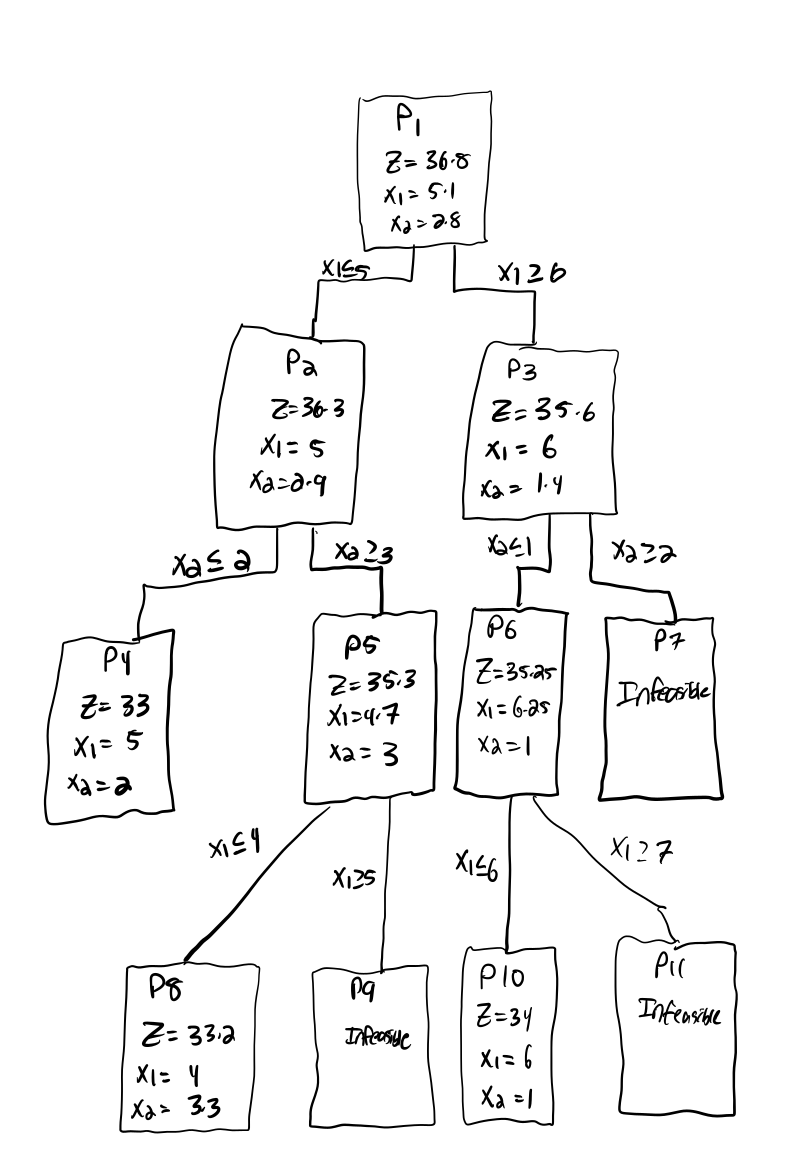
\includegraphics[width=0.9\textwidth]{Prob1-Tree.png}
}

\item Solve the following problem using Branch and Bound
\begin{optprog*}
max & \objective{20 x_1 + 16 x_2 + 25 x_3 + 14 x_4 +9 x_5} \\
st & 3 x_1 + 2 x_2 + 5 x_3 + 4 x_4 + 2 x_5 & \leq & 13 \\
   & x_1, x_2, x_3, x_4, x_5 & \in & \{0,1\}
\end{optprog*}

Solve each subproblem either using python or using the following algorithm:
\begin{itemize}
\item Compute the ratio $r_i$ for each variable where 
\[
r_i = \frac{\text{coefficient of $x_i$ in objective function}}{\text{coefficient of $x_i$ in constraint}}
\]
\item Order $r_i$ from largest to smallest
\item Starting with the largest $r_i$, set $x_i$ to its largest possible (continuous) value without violating the existing constraints.
\end{itemize}

For example, this algorithm to solve the initial problem would compute $r_i$ as:
\[
r_i = \{ \frac{20}{3}, 8, 5 , \frac{7}{2}, \frac{9}{2}\}
\]

The largest of these is $8$ so we would set $x_2 = 1$. The RHS of the constraint is now 11. The next largest is $\frac{20}{3}$, so we would set $x_1 = 1$ and the RHS of the constraint is now 8. The next largest is $5$, so we would set $x_3 = 1$ and the RHS of the constraint becomes $3$. The next largest is $\frac{9}{2}$, so we would set $x_5 = 1$ and the RHS of the constraint becomes $1$. All that's left is $x_4$. We can't set it equal to $1$, instead we maximize it and set $x_4 = \frac{1}{4}$. So the initial solution is $x = (1,1,1,0.25,1)$.

{\blu
This one is very simple. Branch and bound tree is below.

\begin{itemize}
\item Step 1: Solve P1, initial solution is $z = 73.5$ and $x_4$ is fractional. I know $z_{IP} \leq 73$. Branch on $x_4$.
\item Step 2: Solve P2 and P3. For P2, $z = 70$ and $x$ is integral. For P3, $z = 70$ and $x_3$ is fractional. Since P2 is integral, I know $70 \leq z_{I} \leq 73$. Since P3 has a $z = 70$, there's no value in exploring this region. I stop.
\end{itemize}

Optimal solution is $x^* = (1,1,1,0,1)$ with optimal objective function value of $z^* = 70$.

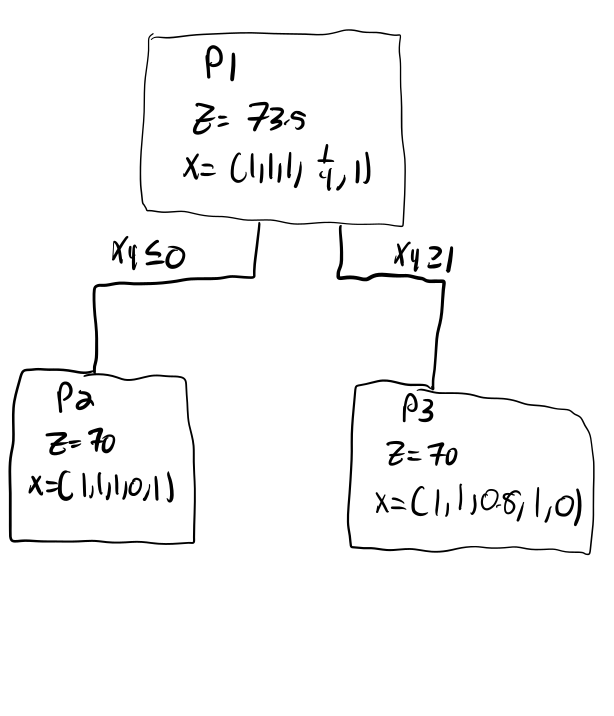
\includegraphics[width = 2.25in]{Prob2-Tree.png}
}

\newpage

\item Solve the following problem using Branch and Bound:

\begin{optprog*}
max & \objective{5 x_1 + 15 x_2 + 12 x_3 + 18 x_4} \\
st & 20 x_1 + 40 x_2 + 30 x_3 + 50 x_4 & \leq & 150 \\
	& x_1 & \leq & 5 \\
	& x_2 & \leq & 3 \\
	& x_3 & \leq & 3 \\
	& x_4 & \leq & 2 \\
   & x_1, x_2, x_3, x_4 & \in & \mathbb{Z}^+
\end{optprog*}

Solve each subproblem either using python or using the same algorithm as problem 2 (notice that this time the variables are not binary so you'd maximize the value based on their upper bounds).

{\blu
Branch and bound tree is on the next page. Steps of the algorithm are as follows.

\begin{itemize}
\item Step 1, solve P1. Initial solution $z = 58.5$, $x_2$ is fractional. At this point, I know $z_{IP} \leq 58$. I can branch on either $x_2$.
\item Step 2, solve P2 and P3. For P2, $z = 58.2$ and $x_4$ is fractional. For P3, $z = 58$, $x_3$ is fractional. I can branch on either P2 or P3. I choose P2 because $58.2 > 58$.
\item Step 3: Solve P4 and P5. For P4, $z = 56$ and solution is integer. For P5, $ z = 57.75$ and $x_2$ is fractional. So at this point, I know $56 \leq z_{IP} \leq 58$. I can choose to branch on either P3 or P5. I choose P3
\item Step 4: Solve P6 and P7. For P6, $z = 57.75$ and $x_2$ is fractional. P7 is infeasible. At this point, my active nodes are P5 and P6. Note that both have the same $z$ value. So I can update my bounds to be $56 \leq z_{IP} \leq 57$. I choose to branch on P5.
\item Step 5: Solve P8 and P9. For P8, $z = 57.6$ and $x_4$ is fractional. For P9, $z = 57$ and $x$ is integral. Note that this means my bound is $57 \leq z_{IP} \leq 57$. This means my current solution is optimal, I can eliminate nodes P8 and P6.
\end{itemize}

Optimal solution is $x^* = (1,1,3,0)$ with optimal objective function value of $z^* = 56$.


\newpage
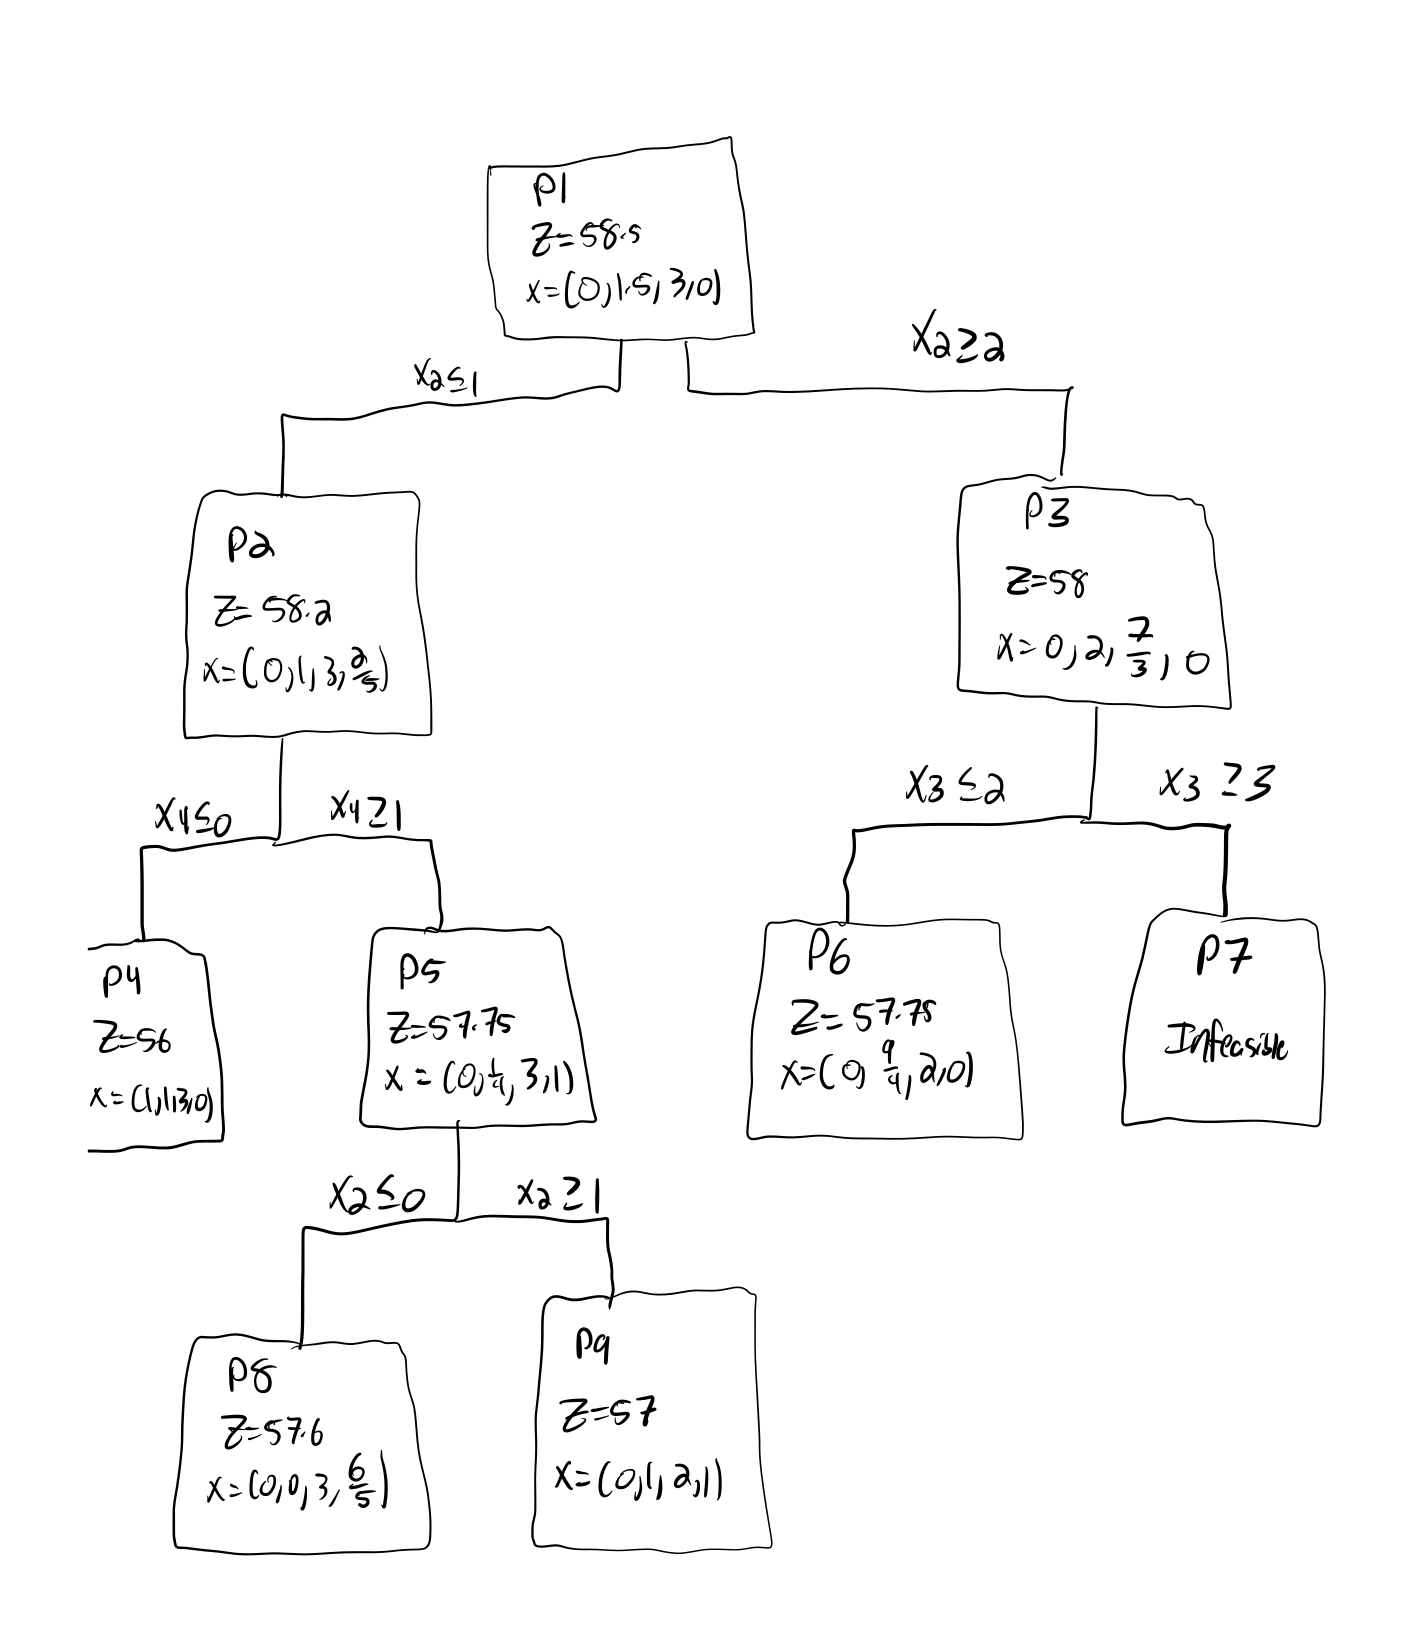
\includegraphics[width=\textwidth]{Prob3-Tree.png}
}

\end{enumerate}




\end{document}
